\setcounter{equation}{0}

\nomenclature{PGAN}{Progressive Generative Adversarial Networks}

\nomenclature{WGAN}{Wasserstein Generative Adversarial Networks}

\nomenclature{SAGAN}{Self-Attention Generative Adversarial Networks}

\nomenclature{CNN}{Convolutional Neural Network}

\nomenclature{GAN}{Generative Adversarial Network}

\nomenclature{ML}{Machine Learning}

\nomenclature{DCGAN}{Deep Convolutional Generative Adversarial Network}

\nomenclature{CGAN}{Conditional Generative Adversarial Networks}

\nomenclature{AI}{Artificial Intelligence}

\nomenclature{FIGAN}{Feature Interpretation Using Generative Adversarial Networks}

\nomenclature{CT}{Computed Tomography}

\nomenclature{MRI}{Magnetic Resonance Imaging}

\nomenclature{MNIST}{Modified National Institute of Standards and Technology}

\nomenclature{DCNN}{Deep Convolutional Neural Network}

\nomenclature{PCA}{Principal Component Analysis}

\nomenclature{PLS}{Partial Least Squares}

\nomenclature{GIF}{Graphics Interchange Format}

\nomenclature{DL}{Deep Learning}

\nomenclature{NN}{Neural Network}

\nomenclature{VAE}{Variational Autoencoders}

\nomenclature{HD}{High Definition}

\nomenclature{BNPP}{B-type Natriuretic Peptide}

\nomenclature{XAI}{Explainable Artificial Intelligence}

\nomenclature{VG}{Visual Geometry}

\nomenclature{Grad-CAM}{Gradient Weighted Class Activation Mapping}

\nomenclature{FID}{Fréchet Inception Distance}

\nomenclature{VAE}{Variational Autoencoder}

\nomenclature{RBM}{Restricted Boltzmann Machine}

\nomenclature{MCMC}{Markov Chain Monte Carlo}

\nomenclature{CAM}{Class Activation Mapping}

\nomenclature{CIU}{Contextual Importance And Utility}

% --------------------------------------------------

\chapter{Introduction}

\noindent Generative Adversarial Networks, commonly known as GANs, are a class of artificial neural networks used in unsupervised machine learning. GANs represent a significant breakthrough in the field of Machine Learning(ML) and Artificial Intelligence(AI). These models were first introduced by Ian J. Goodfellow and his colleagues in 2014\cite{GAN_Main}. As per the creators, GAN is a framework for estimating generative models via an adversarial process\cite{GAN_Main}. GANs have gained prominence in recent years due to their unique ability to generate data that mimics real-world data distributions.

\noindent GANs are conceptually simple in their architecture, but their simplicity contradicts the complexity of the training process and the results they can achieve. The basic GAN architecture consists of just two components: a generator and a discriminator. 

\vspace{2mm}

\begin{figure}[h!]
\centering
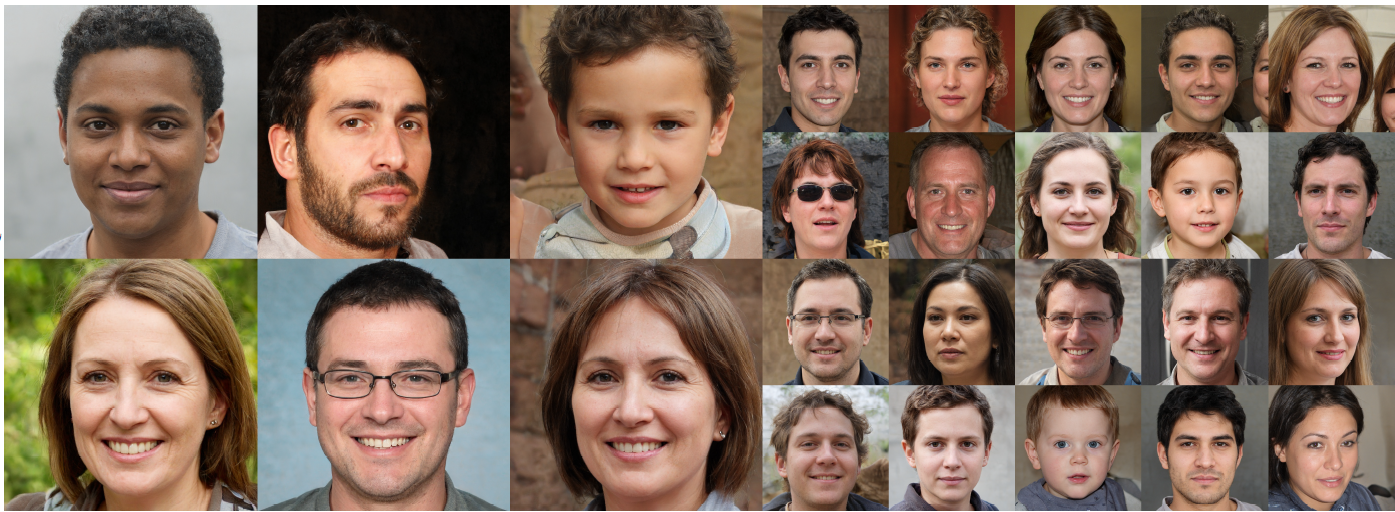
\includegraphics[width=0.7\textwidth]{Images/gan_image_variation.png}
\caption[Random Images generated by a GAN introduced by NVIDIA]{Random Images generated by a GAN created by NVIDIA. The GAN Architecture is known as StyleGAN\cite{StyleGAN}, which generates artificial images starting from a low resolution(noise) to a high resolution. It controls the visual features that are expressed in each level, from coarse features(face shape) to finer details(hair color).}
\end{figure}

\clearpage

\section{Background}

\noindent Before going into the world of Generative Adversarial Networks. We need to understand the whole landscape of artificial intelligence and how GANs came into picture. Figure 2.2 gives the relationship between Artificial Intelligence, Machine Learning, Neural Networks, and Deep Learning.

\begin{wrapfigure}{l}{0.5\textwidth}
    \centering
    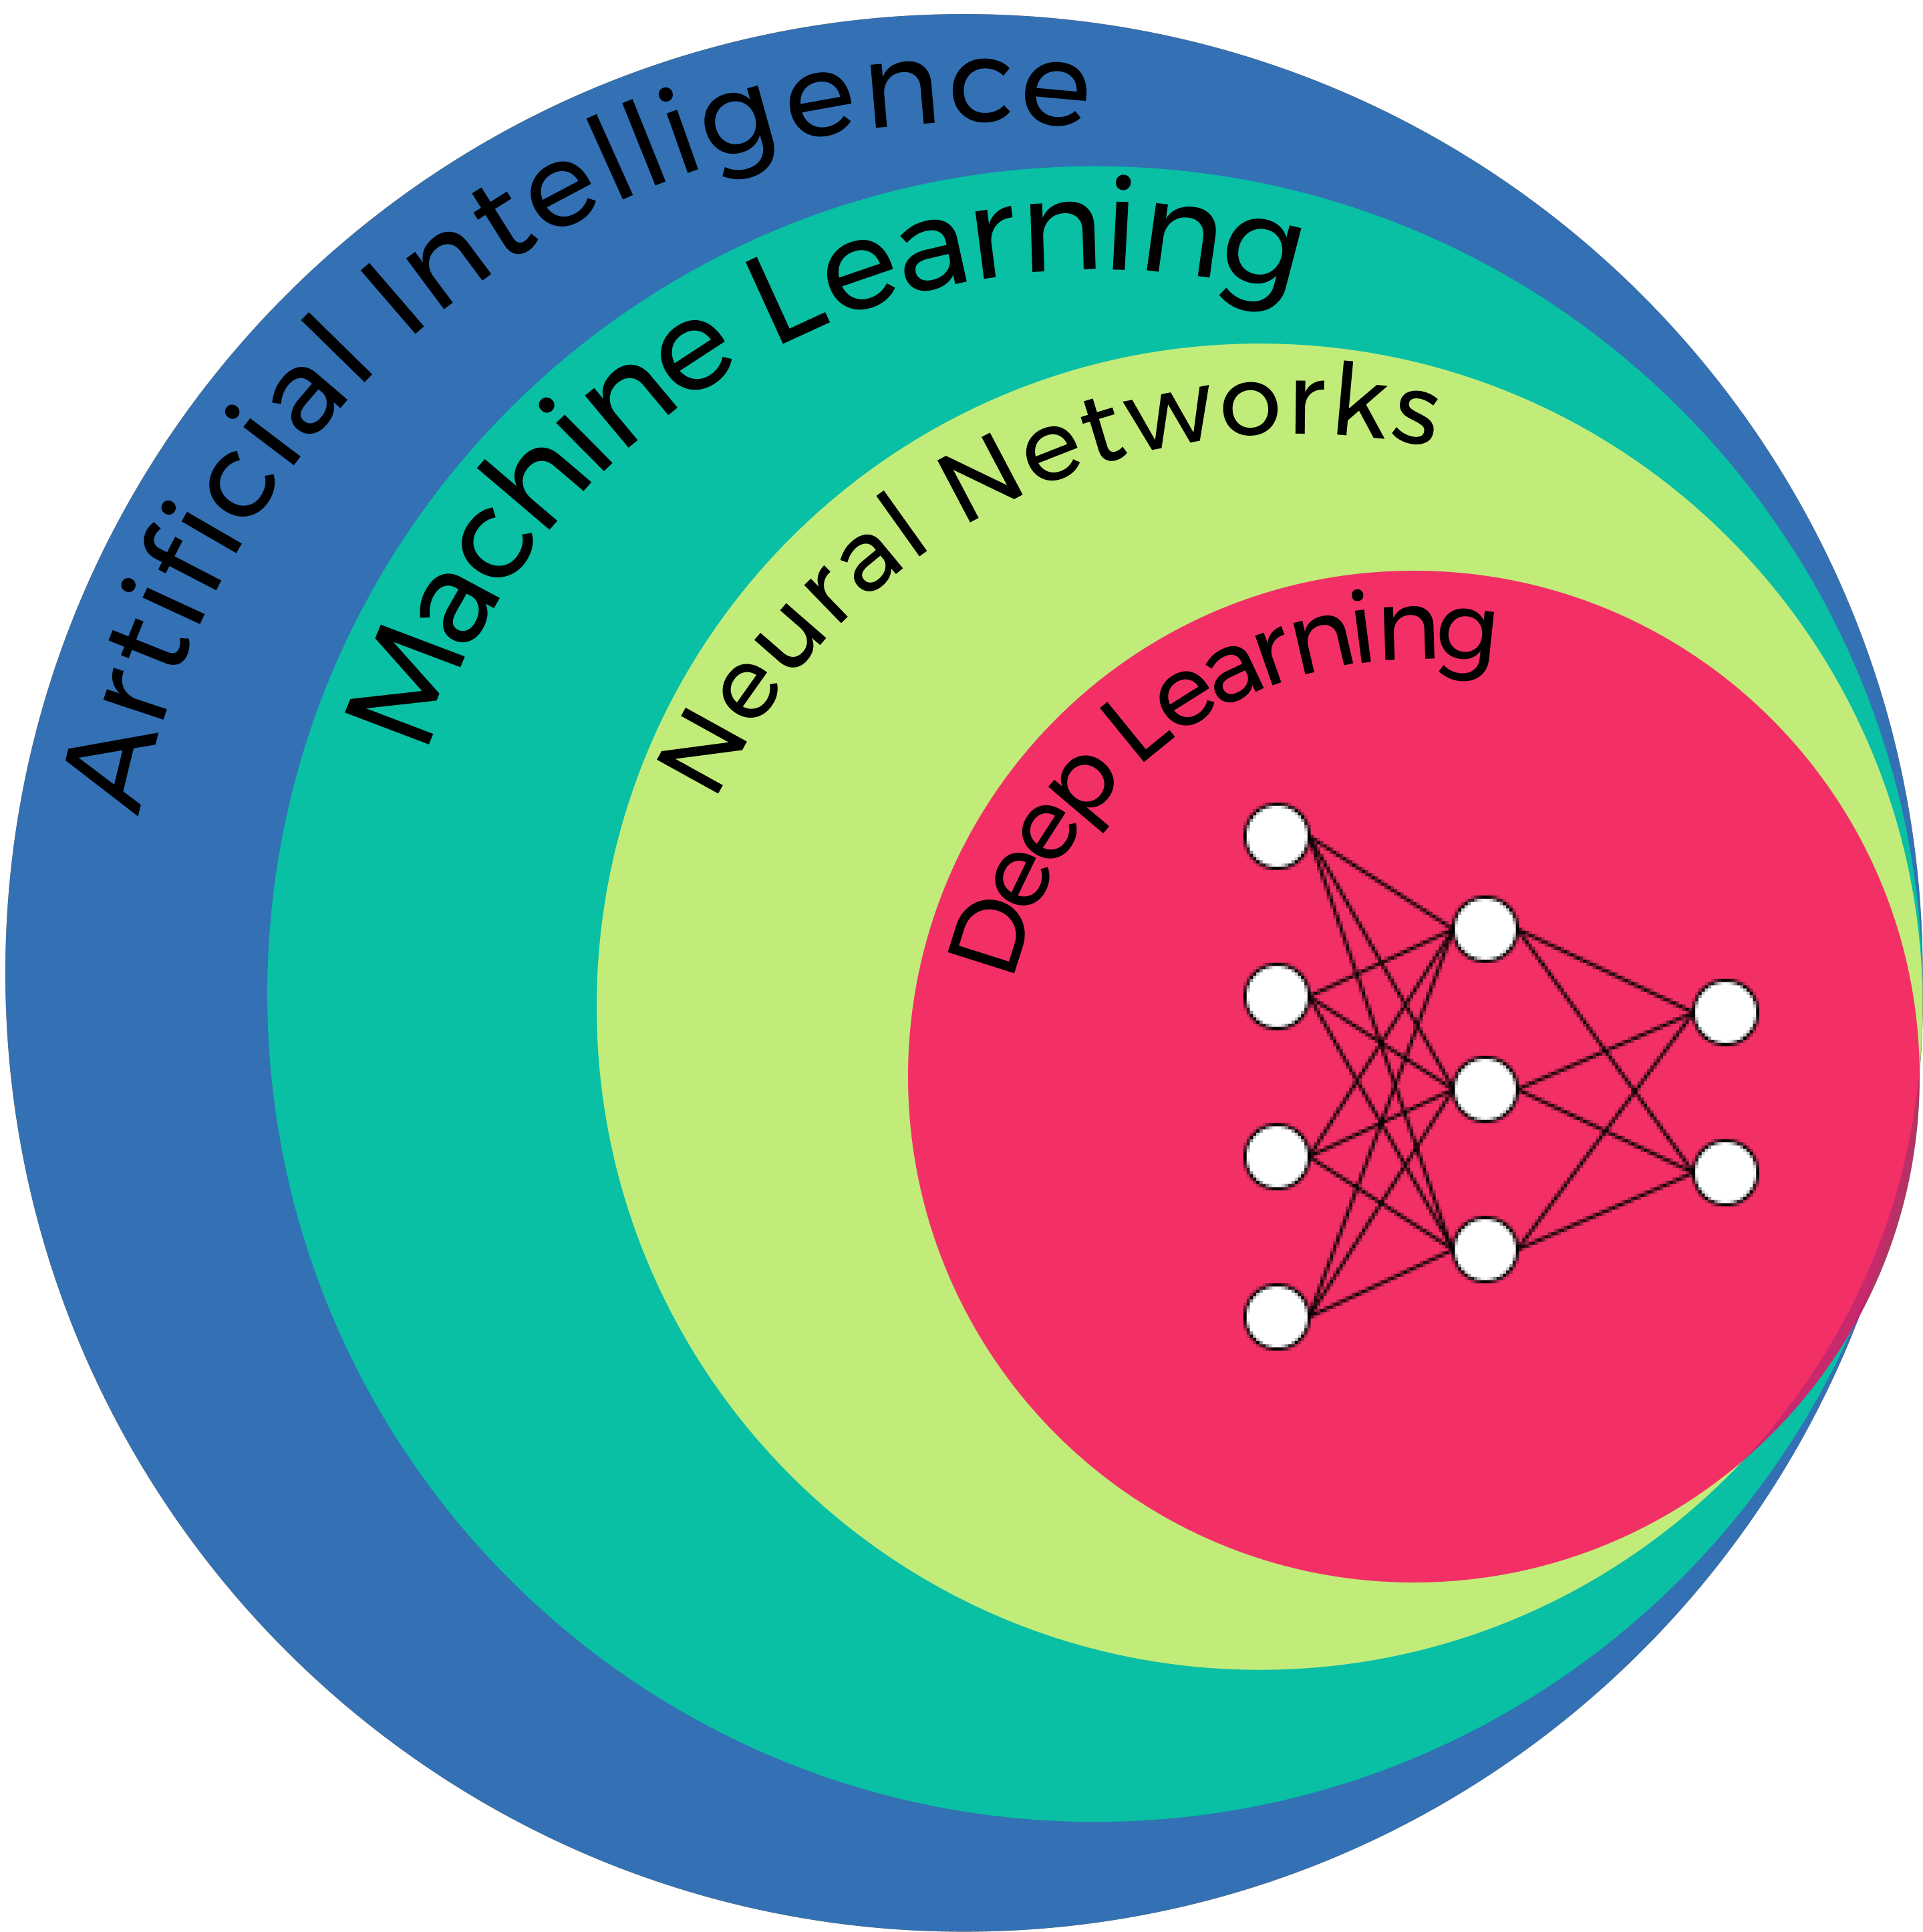
\includegraphics[width=0.3\textwidth]{Images/ai_ml_nn_dl.png}
    \caption[Hierarchy of Artificial Intelligence]{Relationship between AI, \mbox{Machine Learning}, Neural Networks and Deep Learning.}
\end{wrapfigure}

\noindent
Artificial Intelligence is the field of computer science dedicated to creating intelligent agents, that can reason, learn, and act autonomously. Machine Learning is a subfield of AI that combines algorithms that can identify patterns in data without being explicitly programmed. Neural Networks (NNs) are a type of ML algorithm that are made up of interconnected neurons, which are able to learn from data by adjusting the weights between the neuron connections. Deep Learning (DL) is a subfield of ML that uses NNs with multiple layers, and are able to learn from complex data, such as images and languages without defining features explicitly.

\noindent
Figure 2.3 gives a visual idea of how the learning models are arranged. The machine learning models can be broadly classified into supervised learning, unsupervised learning and reinforcement learning.

\begin{figure}[h!]
\centering
\includegraphics[width=0.92\textwidth]{Images/gan_bg.png}
\caption{A visual guide to the taxonomy of learning models.}
\end{figure}

\clearpage

\noindent
Supervised learning is a type of ML in which the data provided for learning has labels(ground truths) in it. It is divided into regression and classification tasks, in which neural networks are commonly used in both tasks, thereby researchers have derived a new branch(or subset) of machine learning which is called Deep Learning.

\noindent
The Deep Learning models can be broadly categorized into two main types: Generative Models and Discriminative Models.

\begin{itemize}
    \item \textbf{Generative Models:}
    \begin{itemize}
        \item Generative models are designed to model the underlying probability distribution of a dataset\cite{GenAI}. They generate new data points that are similar to the training data they were exposed to. Generative models are often used for tasks such as image generation, text generation, and data synthesis.\\
        One of the best examples of a generative deep learning model is GANs - An unsupervised generative machine learning model that can create new and realistic data based on its training data.
    \end{itemize}

    \item \textbf{Discriminative Models:}
    \begin{itemize}
        \item Discriminative models, on the other hand, aim to learn the boundary or decision surface that separates different classes or categories in the data. They are typically used for classification and regression tasks.\\
        One of the best examples of a discriminative deep learning model is Convolutional Neural Networks - A model used for classification and other image and audio related tasks in deep learning.
    \end{itemize}
\end{itemize}

\clearpage

\section{Motivation}

\noindent The motivation behind studying GANs lies in their transformative potential in various domains and GANs are considered to be one of the earliest and most effective applications of Generative AI when it comes to real discussions. And GANs also have the power to:

\begin{itemize}
    \item Generate realistic images, text, and even videos:
        \begin{itemize}
            \item The work on generating realistic data represents a profound advancement in computer vision and natural language processing.
            \item This could even help in industries such as photography, and movies by generating high-quality images and videos that could be used as fillers in their works.
            \item Realistic images and videos could be used to make artificial environments, where we could train reinforcement models and create video games.
        \end{itemize}
        
    \item Aid in data augmentation and synthesis, benefiting healthcare\cite{Data_Aug}, finance\cite{CORRGAN}, and many other industries.
        \begin{itemize}
            \item GANs can generate synthetic medical images, such as X-rays, Computed Tomography(CT) scans, or Magnetic Resonance Imaging(MRI) images, which can be used for training and testing machine learning models. This is especially helpful when there is a scarcity of labeled data.
            \item GANs can generate normal patient data, allowing healthcare organizations to train models for anomaly detection, such as identifying rare diseases or unusual medical conditions.
            \item GANs can generate molecular structures, aiding in the discovery of new drugs by simulating various chemical compounds. This can accelerate the drug development process and reduce costs.
        \end{itemize}
\end{itemize}

\noindent
GANs stand as a pivotal innovation with profound implications across diverse sectors like visual media, data synthesis, and problem-solving. The transformative potential of GANs in augmenting creativity and addressing complex problems underscores GAN being the focal point of this seminar.

\clearpage

\section{Outline}

\noindent
The outlined structure delves deeply into Generative Adversarial Networks and their diverse applications. It starts with an introduction that sets the stage for understanding GANs and proceeds with a comprehensive exploration of their historical journey, tracing their evolution with insights gained from extensive research writings on the subject. This study helps in understanding how GANs have developed and transformed over time.

\noindent
Moving forward, the report takes a closer look at the fundamental components of GANs, breaking down complex concepts into more digestible bits. It details their architecture, explaining how they're built, the methods used to train them, and the various types that exist. By unraveling these aspects, the aim is to simplify the understanding of how GANs function and their different variations.

\noindent
Furthermore, the report dives into the methodologies used by researchers to study GANs, shedding light on the processes involved in gathering important data. It explores the theories behind GANs, aiming to identify areas where further research could be fruitful. This section also focuses on making AI systems easier to comprehend, highlighting the limitations of current methods and proposing a new approach called FIGAN that aims to enhance the clarity of AI systems.

\noindent
In addition to theoretical discussions, the report describes frameworks employed in addressing a critical aspect, AI explainability. Which scrutinizes widespread limitations or doubt about how AI systems make decisions, and introduces innovative methodologies, the FIGAN architecture, to enhance explainability within AI systems.

\noindent
Lastly, the conclusion sums up the accumulated insights, acknowledging the existing limitations in understanding GANs while pointing out potential avenues for future research and innovation. It acts as a guide for further exploration and improvement in the field of Generative Adversarial Networks.